\documentclass[a4paper,10pt,twoside]{article}
\usepackage[italian]{babel}
\usepackage[utf8x]{inputenc}
\usepackage{amsmath}
\usepackage{amsthm}
\usepackage{amssymb}
\usepackage{amscd}
\usepackage{graphicx}
\newtheorem{defi}{Definizione}
\newtheorem{teo}{Teorema}
\newtheorem{cor}{Corollario}
\newtheorem{note}{Nota}
\newtheorem{es}{Esercizio}
\parindent=0cm
\thispagestyle{empty}
\usepackage[font=sf, labelfont={sf,bf}, margin=1cm]{caption}

\begin{document}

{\Large Determinazione della velocità del suono}

\vspace{2cm}
La prima determinazione analitica della velocità del suono venne data da Isaac Newton nella proposizione 49 del libro II dei Principia. Per dell'aria a pressione di una atmosfera e temperatura di 25°C Newton calcolò una velocità di circa $297 ms^{-1}$, un valore più basso di circa il 15\% rispetto a quello reale di circa $343ms^{-1}$. Fu, più tardi, Laplace a correggere il ragionamento di Newton e a calcolare in maniera molto più accurata la velocità del suono in aria. Il metodo di Newton era essenzialmente corretto, e lo stesso Laplace ammise che l'analisi del suo famoso precursore era un ``monumento al suo grande genio''.
Consideriamo un tubo all'interno del quale si propaga un impulso di pressione come mostrato in figura[\ref{tubo}].
\begin{figure}[h]
 \begin{center}
  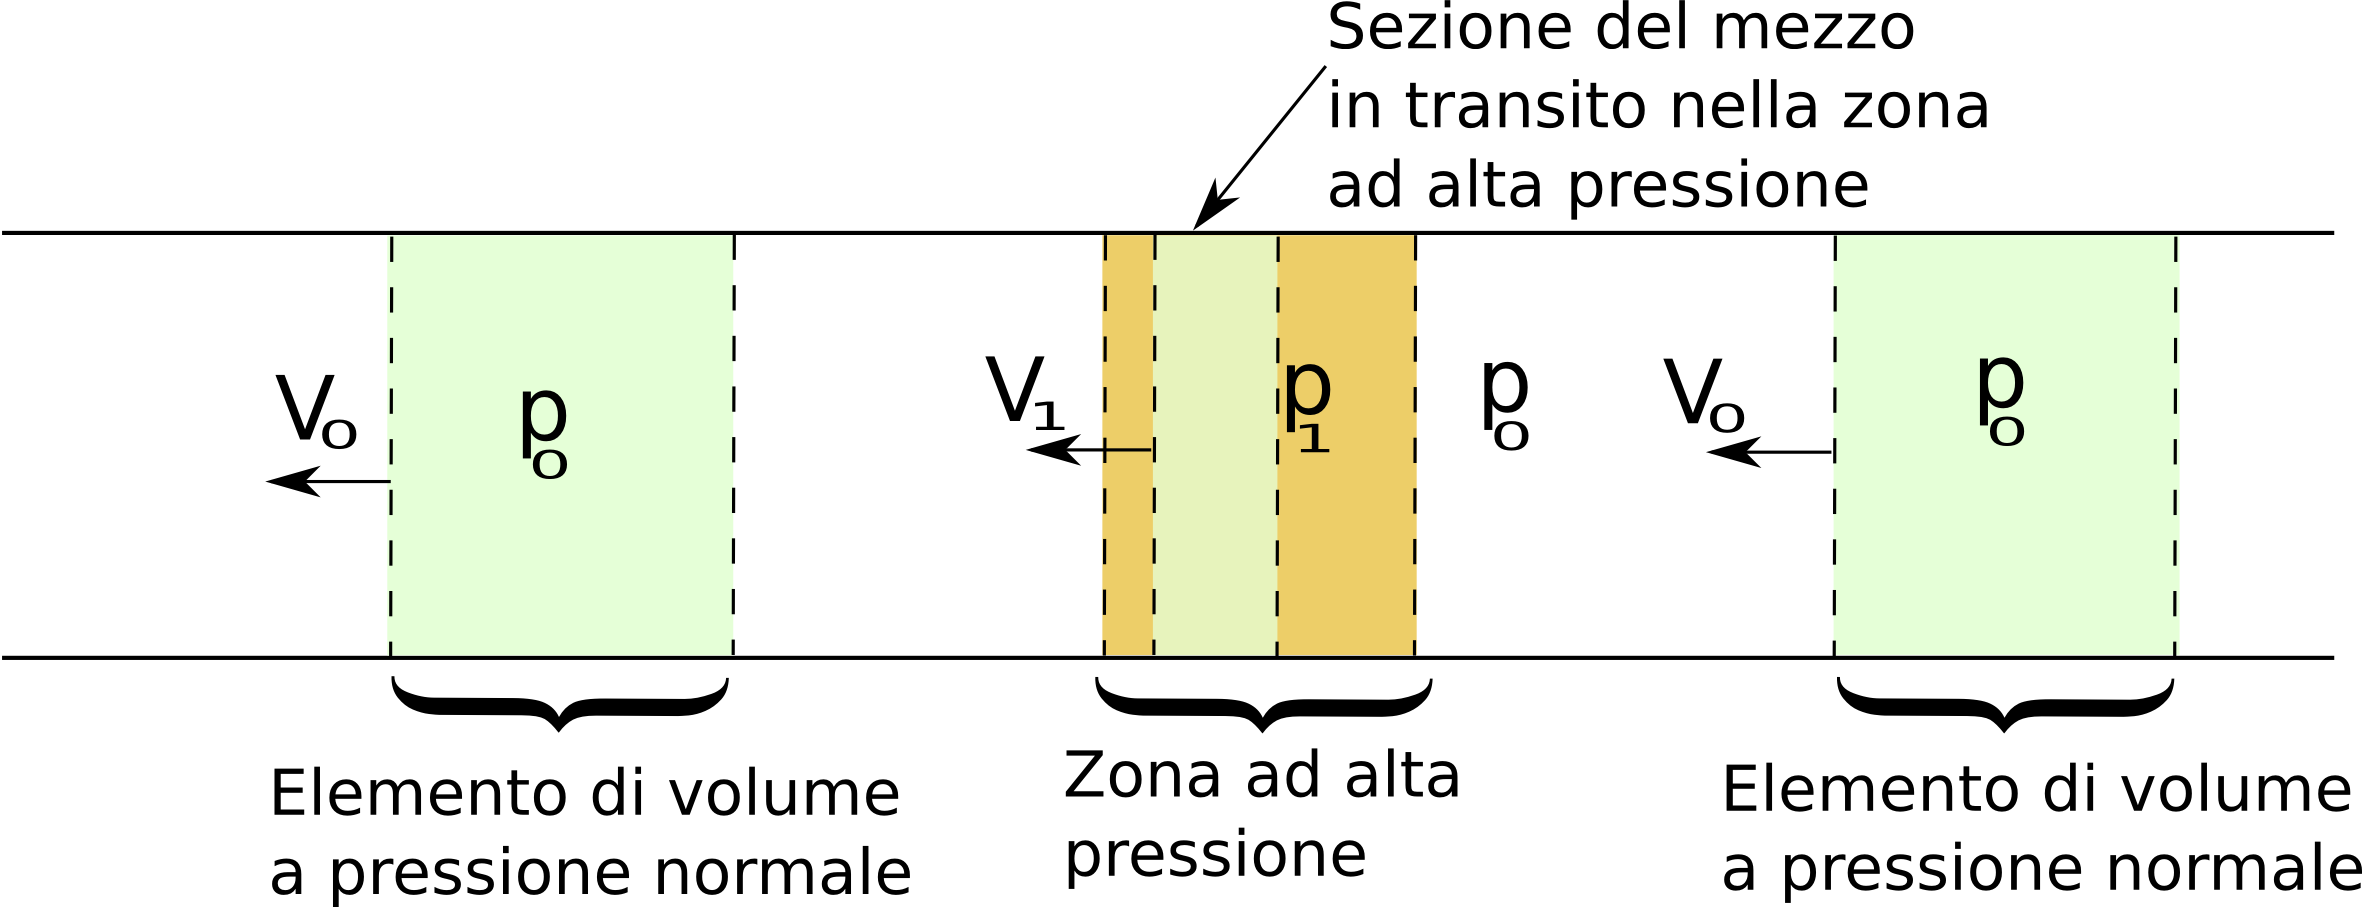
\includegraphics[width=0.8\textwidth]{tubo1.png}
 \caption{Un impulso di pressione si propaga all'interno di un tubo, per un osservatore solidale con l'impulso questo è fermo e il mezzo lo attraversa}\label{tubo}
\end{center}
\end{figure}
Per determinare la velocità alla quale un'onda piana di pressione  si propaga all'interno di un mezzo, schematizziamo   l'impulso di pressione con una funzione a scalino scalino nel piano $(x,p)$ \footnote{Riportiamo in ascissa la posizione ed in ordinata la pressione associata a quel punto del tubo} come  mostrato in figura [\ref{scalino}]:
\begin{figure}[h]
\begin{center}
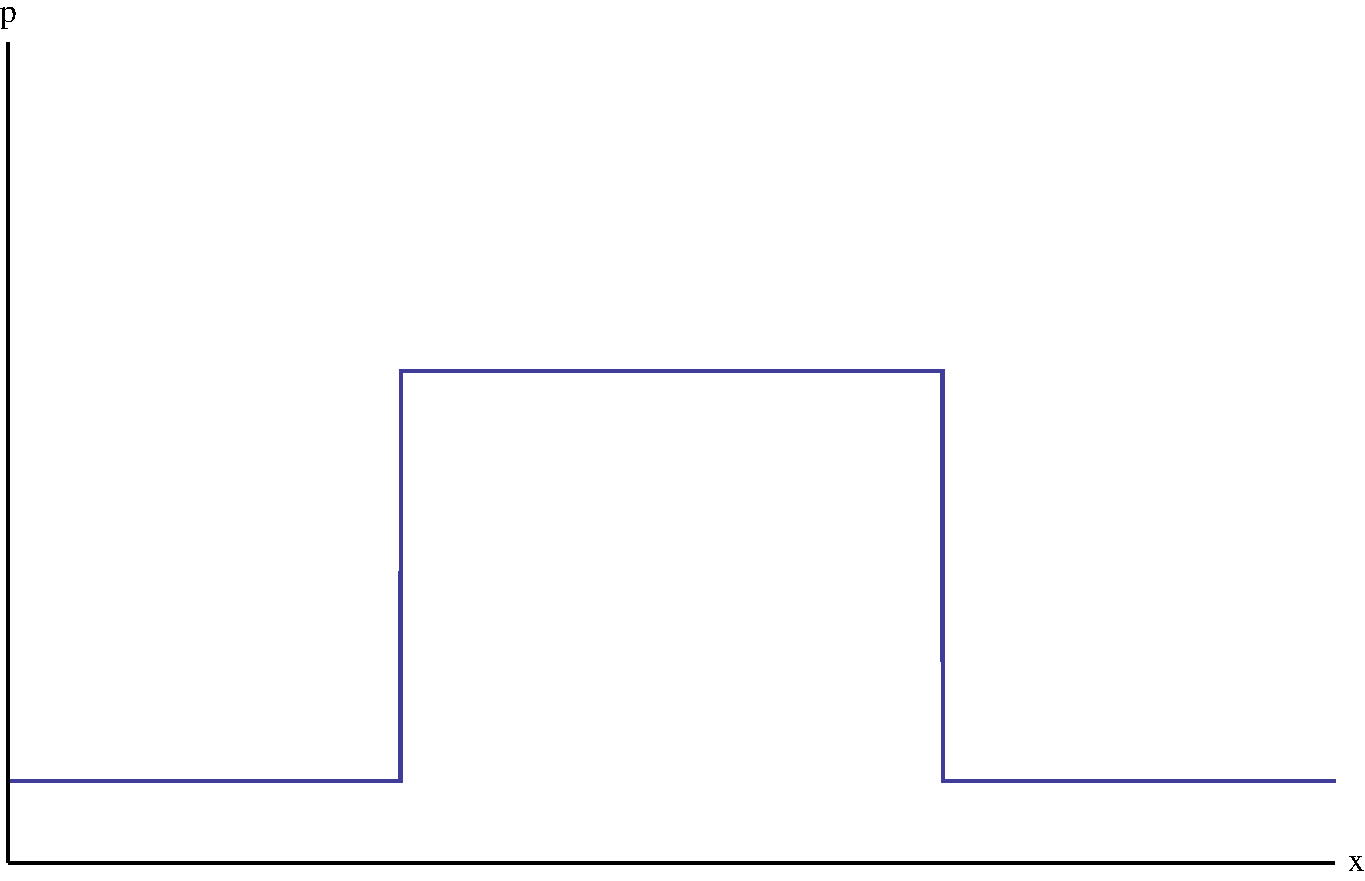
\includegraphics[width=0.8\textwidth]{pressione1.pdf}
\end{center}\caption{Un impulso a scalino di pressione che si propaga verso destra con velocità $\mathbf{v_0}$}\label{scalino}
\end{figure}
possiamo immaginare che questo impulso di pressione si propaghi verso destra con una velocità $\mathbf{v_0}$, per semplificare la trattazione considereremo un sistema di riferimento solidale con l'impulso di pressione. In tale sistema l'impulso stesso è immobile e il mezzo si sposta verso sinistra con velocità in modulo $v_0$. 
\begin{figure}[h]
 \begin{center}
  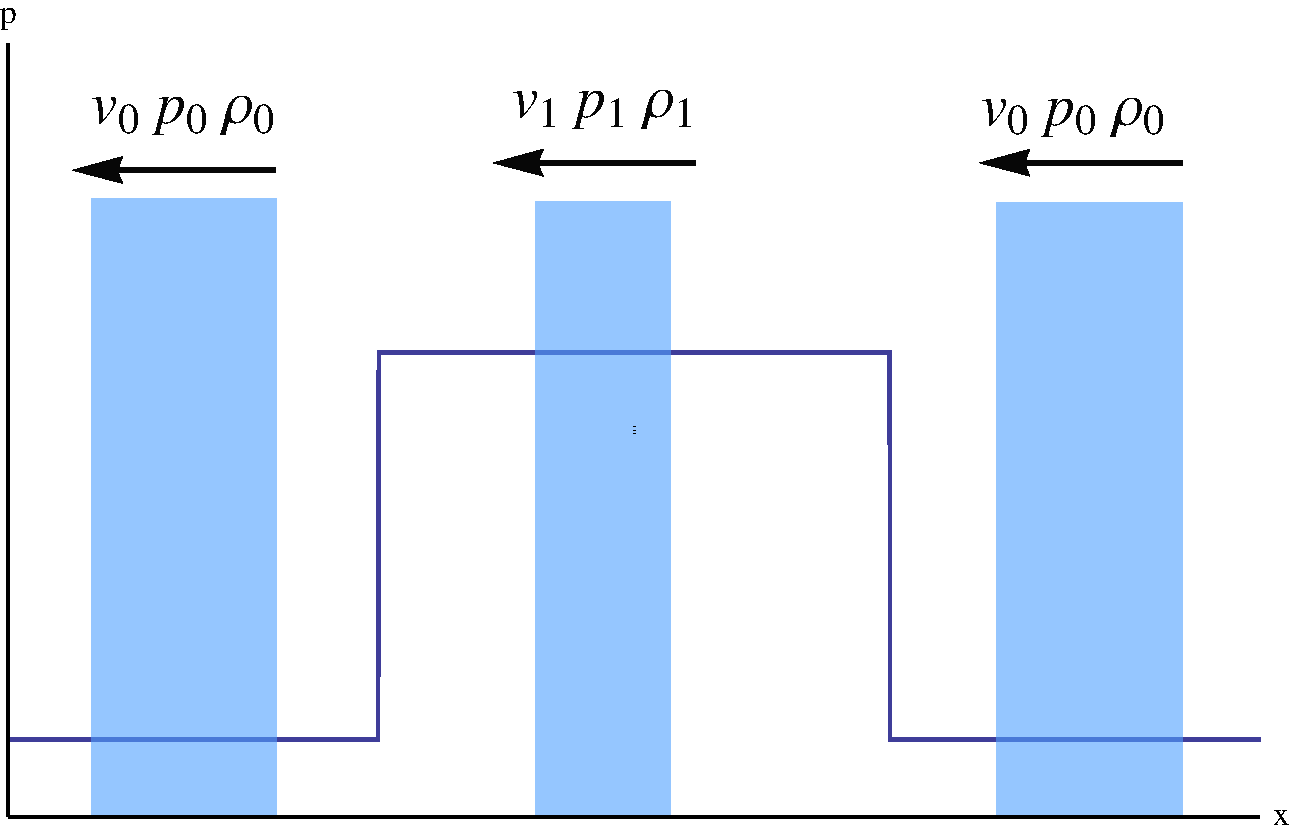
\includegraphics[width=0.8\textwidth]{pressione2.pdf}
 \end{center}
\caption{Nel sistema di riferimento solidale all'impulso il mezzo si sposta verso sinistra con velocità in modulo $v_0$}\label{mezzo}
\end{figure}
Nella figura [\ref{mezzo}] sono rappresentate tre zone del mezzo all'interno del quale si propaga l'impulso di pressione aventi la stessa massa, una si sta avvicinando all'impulso, una si trova all'interno dell'impulso e la terza ha già oltrepassato l'impulso. Siccome all'interno dell'impulso la densità è maggiore, la continuità del flusso ( ovvero la quantità di materia che entra all'interno dell'impulso di pressione deve essere la stessa di quella che ne è uscita) richiede che la velocità del mezzo all'interno dell'impulso stesso sia minore che all'esterno. Il mezzo deve quindi decellerare quando entra nell'impulso e acellerare quando lo lascia.
Focalizziamo ora la nostra attenzione su una sezione del mezzo che sta per entrare nella zona ad alta pressione e densità (l'impulso) come mostrate nella figura [\ref{entra}]
\begin{figure}[h]
\begin{center}
 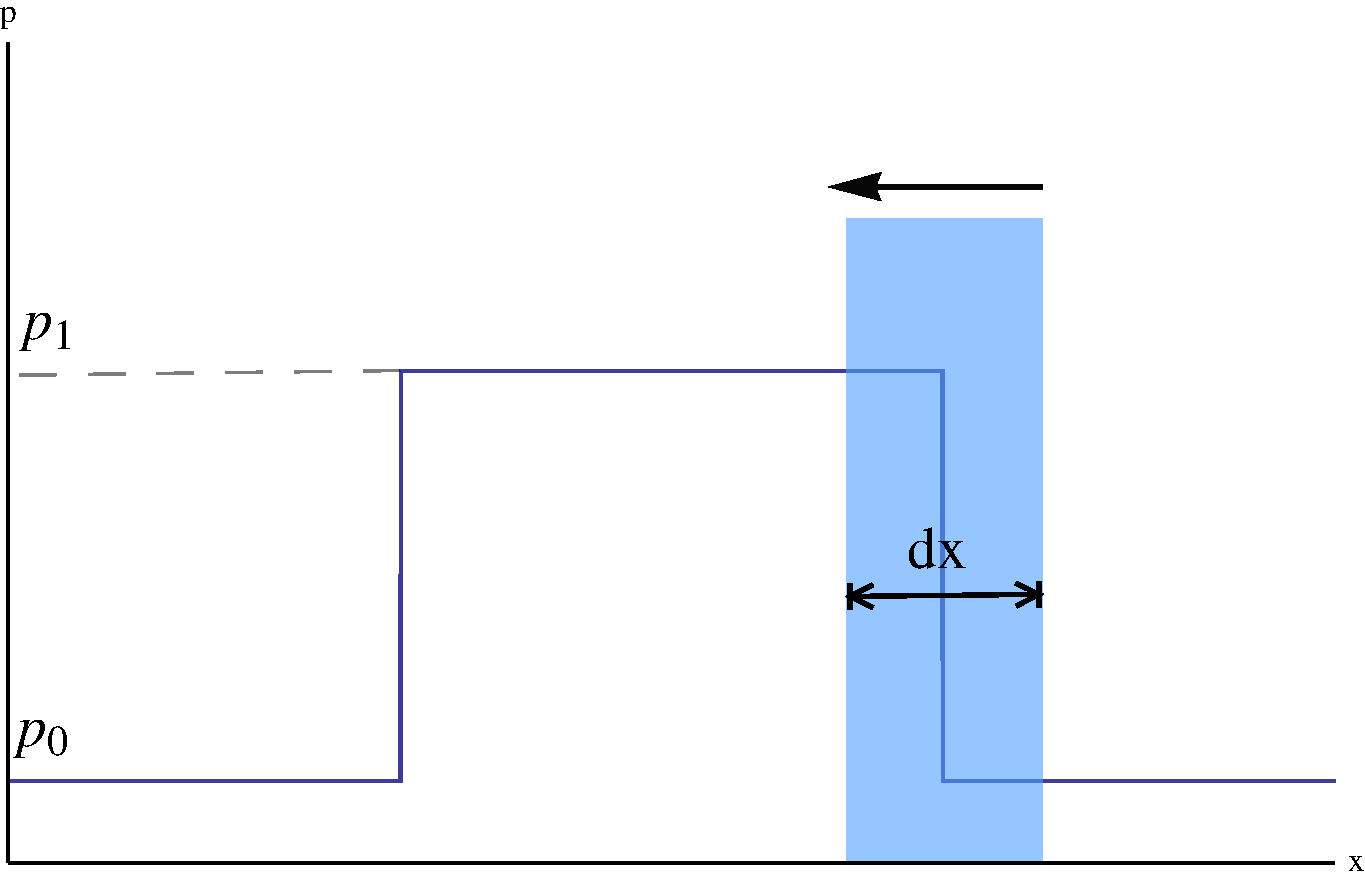
\includegraphics[width=0.8\textwidth]{pressione3.pdf}
\end{center}
 \caption{Una sezione del mezzo di spessore $dx$ entra all'interno della zona ad alta pressione e densità}\label{entra}
\end{figure}
La superficie più avanzata di questa sezione è appena entra nella zona critica (l'impulso), è quindi soggetta alla pressione $p_1$, mentre la superficie più arretrata della sezione si trova ancora nella zona di spazio a pressione ordinaria  $p_0$. La differenza di pressione produce una forza netta per unità di superficie pari a $p_1-p_0$ verso destra, ovvero questa forza decelera il mezzo entrante nella zona ad alta densità. Questa forza è applicata per un tempo $dt$, il tempo necessario alla sezione del mezzo  ad oltrepassare l'interfaccia tra la zona a bassa pressione e quella ad alta pressione. Siccome la velocità del mezzo è in modulo $v_0$ il tempo $dt$ è: 
\begin{equation}\label{tempo}
 dt=dx/v_0
\end{equation}
Applicando ora la seconda legge di Newton $\mathbf{F}=m\mathbf{a}$ alla sezione di gas presente all'interno del tubo e propagantesi attraverso la regione ad alta pressione e notando che:
\begin{itemize}
 \item la forza per unità di superficie che decelera la sezione è $p_1-p_0$
\item la massa per unità di superficie è $\rho_0dx$ dove $\rho_0$ è la densità del mezzo nella zona a bassa pressione
\item l'accelerazione cui è soggetta la sezione del mezzo che attraversa l'interfaccia con la zona ad alta pressione è ($v_0-v_1)/dt$
\end{itemize}
otteniamo:
\begin{equation}\label{pass1}
 p_1-p_0=\rho_0dx\frac{v_0-v_1}{dt}
\end{equation}
sostituendo la [\ref{tempo}] nella [\ref{pass1}] otteniamo:
\begin{equation}
 p_1-p_0=\rho_0v_0(v_0-v_1)
\end{equation}

La continuità del flusso per unità di superficie (ovvero la materia che entra nell'unità di tempo all'interno della zona ad alta pressione deve essere la stessa che ne esce) richiede che il prodotto della velocità e della densità sia costante:
\begin{equation}\label{flusso}
\rho_0v_0=\rho_1v_1
\end{equation}
sottraendo $\rho_1v_0$ ad ambo i membri della [\ref{flusso}] otteniamo:
\begin{equation}
 \frac{v_0}{\rho_1}(\rho_1-\rho_0)=v_0-v_1
\end{equation}
che sostituita nella [\ref{pass1}] ci da:
\begin{equation}\label{vel1}
 v_0^2=\frac{\rho_1}{\rho_0}\left(\frac{p_1-p_0}{\rho_1-\rho_0}\right)
\end{equation}

nel limite di piccole variazioni della pressione (che rappresenta un'ottima approssimazione per le onde sonore) il rapporto $\rho_1/\rho_0$ tende ad $1$ ed otteniamo il risultato di Newton:
\begin{equation}\label{veldef}
 v_0=\sqrt{\frac{p_1-p_0}{\rho_1-\rho_0}}=\sqrt{\frac{\Delta p}{\Delta \rho}}=\sqrt{\frac{B}{\rho_0}}
\end{equation}
 dove abbiamo definito il modulo di elasticità cubica del mezzo come:
\begin{equation}
 B=\rho_0 \frac{\Delta p}{\Delta \rho}=-V\frac{\Delta p}{\Delta V}
\end{equation}
Per determinare ora la velocità del suono in aria ( o in altri gas ideali) dobbiamo conoscere come pressione e densità sono correlate. Newton era a conoscenza della legge di Boyle (a temperatura costante la densità di un gas è proporzionale alla pressione) che espressa attraverso la legge dei gas ideali ci dice:
\begin{equation}
 p=\rho RT
\end{equation}
dove $R$ è la costante universale dei gas. Da questa legge deduciamo facilmente come $dp/d\rho=RT$ Inserendo questa relazione nella [\ref{vel1}] otteniamo:
\begin{equation}\label{vel2}
 v_0=\sqrt{RT}
\end{equation}
Il semplice calcolo effettuato non è corretto, calcolando, infatti, per un gas perfetto a temperatura costante il modulo di elasticità cubica otteniamo:
\begin{equation}
 \rho\frac{dp}{d\rho}=\rho RT=P
\end{equation}
che sostituito nella [\ref{veldef}] ci permette di dire:
\begin{equation}
 v_0=\sqrt{\frac{P}{\rho_0}}
\end{equation}
nel caso dell'aria a pressione di una atmosfera $p=10^5Nm^2$ e densità $\rho=1.29 kgm^{-3}$ otteniamo per la velocità  del suono un valore :
\begin{equation}
 v\simeq 278ms^{-1}
\end{equation}
valore di circa il $18\%$ inferiore rispetto a quello reale. Il motivo della discrepanza con i dati sperimentali è da ricercarsi nella non costanza della temperatura dell'aria al passare della perturbazione di pressione. Quando studieremo le trasformazioni adiabatiche illustreremo l'estensione di Laplace al metodo di Newton per il calcolo della velocità del suono. 


 
 
\end{document}
